\documentclass[aps,prl,twocolumn,superscriptaddress,showpacs,floatfix]{revtex4-2}

\usepackage{graphicx}
\usepackage{amsmath}
\usepackage{amssymb}
\usepackage{hyperref}
\usepackage{bm}
\usepackage{tikz}
\usetikzlibrary{decorations.pathmorphing,decorations.pathreplacing,arrows.meta,positioning,calc,backgrounds,fit}

\newtheorem{proposition}{Proposition}

\newcommand{\Tr}{\mathrm{Tr}}
\renewcommand{\vec}[1]{\boldsymbol{#1}}
\newcommand{\ket}[1]{|#1\rangle}
\newcommand{\bra}[1]{\langle#1|}

\begin{document}

\title{Equilibrium from the Inside Out: Exact Hamiltonian of Mean Force}
\author{Gerard McCaul}
\date{\today}

\begin{abstract}
We ask when the reduced equilibrium state of an open quantum system can be
written not merely as an implicit density operator but as an explicit
Hamiltonian-level generator. Starting from the quenched representation of the
traced Gibbs state, we derive an exact Gaussian reformulation in which bath
physics enters through scalar kernel moments while operator growth is carried
entirely by the adjoint chain generated by the bare Hamiltonian and the
coupling. The exact Gaussian HMF therefore comes with a compositional
architecture of its own: an adjoint orbit, a bilinear influence aggregation,
and a nonlinear Baker--Campbell--Hausdorff recombination. This yields a
closure criterion: a finite closed-form Hamiltonian of mean force exists only
when that operator family closes inside the chosen ansatz. For the spin-boson
qubit all three layers close exactly, yielding, to our knowledge, the first
closed-form HMF for a genuinely noncommuting open quantum system. The same
variables organize the numerical crossover: once the dressed state outgrows
the available basis, simulation error reflects a representability bottleneck
rather than a breakdown of the exact theory. The resulting perspective treats
strong-coupling equilibrium as a problem of constructive reduced description,
compact operator classes, and finite-resource inference.
\end{abstract}

\maketitle

\section{Introduction}
\label{sec:intro}

A central question of equilibrium quantum statistical mechanics is what
survives coarse-graining. Before reduction, equilibrium is generated by a
Hamiltonian and written $\rho\propto e^{-\beta H}$: the state and its generator
are given together. After an environment is traced out, the reduced
equilibrium state remains well defined, but the generator need not remain
transparent. The sharper question is therefore not whether reduced equilibrium
exists, but whether it can still be written as an explicit Hamiltonian rather
than only as an implicit density operator. This is the inside-out version of
equilibrium, where one starts from the reduced state and asks what generator,
if any, survives the reduction.

For an open system with finite coupling, the operational equilibrium state of
the subsystem is the reduced state of the global Gibbs ensemble,
\begin{align}
    \bar{\rho}_Q(\beta) &= \Tr_X\, e^{-\beta H_{\mathrm{tot}}},
    \label{eq:intro_rho_bar} \\
    e^{-\beta H_{\mathrm{MF}}(\beta)}
    &\propto \frac{\Tr_X e^{-\beta H_{\mathrm{tot}}}}{Z_X(\beta)},
    \qquad Z_X(\beta)=\Tr_X e^{-\beta H_X}.
    \label{eq:intro_hmf_def}
\end{align}
The Hamiltonian of mean force (HMF) is the operator that restores a Gibbs-form
description after the bath has been traced out. It is therefore the exact
reduced equilibrium generator whenever system--bath coupling is finite
\cite{campisiFluctuationTheoremArbitrary2009,talknerColloquiumStatisticalMechanics2020,trushechkinOpenQuantumSystem2022,seifertFirstSecondLaw2016,campbellRoadmapQuantumThermodynamics2026,binderThermodynamicsQuantumRegime2018}.

Why care about a mean-force Hamiltonian at all? First, it underlies the
free-energy, work, and entropy relations of strong-coupling thermodynamics
\cite{jarzynskiNonequilibriumWorkTheorem2004,campisiFluctuationTheoremArbitrary2009,seifertFirstSecondLaw2016,millerEntropyProduction2017,lacerdaQuantumThermodynamicsFast2023,BinderVinjanampathyModiGoold2015}.
Second, it provides a consistent reduced equilibrium state when correlations
with the environment cannot be ignored
\cite{pechukasReducedDynamicsNeed1994b,trushechkinOpenQuantumSystem2022,gelinThermodynamicsSubensembleCanonical2009a}.
Third, and more conceptually, it turns a traced Gibbs operator into a
constructive reduced description that can be inspected, truncated, or compared
across operator families.

That constructive viewpoint matters whenever reduced descriptions must remain
explicit, interpretable, or computationally tractable. Recent work on
representation cost emphasizes that coarse-graining is constrained by what a
reduced model class can continue to carry~\cite{mccaulCostComplexity2026}. A
parallel instinct now appears in machine learning through compact
compositional architectures such as Kolmogorov--Arnold networks, which ask
when complicated multivariate dependence can still be carried by a structured
low-complexity decomposition~\cite{liuKANKolmogorovArnoldNetworks2024}. We
return to that comparison only after the physics problem has been made
precise. The present paper remains entirely about equilibrium statistical
mechanics: given an exact reduced Gibbs state, when does it stay inside a
compact operator family?

The literature is broad but structurally clear. Canonical definitions and
thermodynamic identities are now well established
\cite{campisiFluctuationTheoremArbitrary2009,jarzynskiNonequilibriumWorkTheorem2004,seifertFirstSecondLaw2016,talknerColloquiumStatisticalMechanics2020,trushechkinOpenQuantumSystem2022}.
Exact evaluations exist in special cases: commuting interactions close
trivially, quadratic models preserve Gaussianity, and finite-dimensional
examples such as the spin-boson model provide controlled testbeds
\cite{campisiTalknerHanggi2009Solvable,caldeiraQuantumTunnellingDissipative1983a,grabertQuantumBrownianMotion1988,hiltHamiltonianMeanForce2011,leggettDynamicsDissipativeTwostate1987}.
Benchmark asymptotes in weak coupling and in strongly dressed regimes are also
known and remain important checks on any exact construction
\cite{cresserWeakUltrastrongCoupling2021a,hovhannisyanHamiltonianMeanForce2020}.
Recent work has further emphasized operator structure, bath feedback, and
finite-reservoir generalizations
\cite{burkeStructureHamiltonianMean2024,correaPotentialRenormalisationLamb2025,duGeneralizedHamiltonianMeanforce2025a}.

Outside solvable models, however, the HMF is usually accessed numerically or
perturbatively. Reaction-coordinate mappings, polaron transforms, hierarchical
equations, stochastic approaches, and direct imaginary-time solvers can compute
$\bar\rho_Q(\beta)$, but they rarely return a compact closed-form generator
\cite{nazirReactionCoordinateMapping2018,IlesSmithDijkstraLambertNazir2016,AntoSztrikacsNazirSegal2023,ShubrookIlesSmithNazir2025,moixEquilibriumreducedDensityMatrix2012,chenRigorousStochasticMatrix2014,makriExploitingClassicalDecoherence2014,tanimuraReducedHierarchicalEquations2014,songCalculationCorrelatedInitial2015,XuVadimovStockburgerAnkerhold2026,stockburgerSimulatingSpinbosonDynamics2004,mccaulPartitionfreeApproachOpen2017c}.
The obstruction is therefore not the existence of the reduced equilibrium state
but its representability: when does the logarithm of a traced exponential stay
inside a restricted operator family such as few-body terms, local operators, or
a chosen algebra?

The influence-functional formalism is a natural language for this question. For
Gaussian baths with linear coupling it provides an exact route to integrating
out environmental degrees of freedom
\cite{feynmanTheoryGeneralQuantum1963a,caldeiraQuantumTunnellingDissipative1983a,grabertQuantumBrownianMotion1988}.
In equilibrium it becomes an imaginary-time influence functional, which admits
a Hubbard--Stratonovich rewriting as a quenched stochastic average
\cite{hubbardCalculationPartitionFunctions1959a,stratonovich1957QDistro,stockburgerExactNumberRepresentation2002}.
This formulation makes the reduction step explicit: the partial trace becomes
an average over imaginary-time back-action histories, while all remaining
questions are pushed onto the system operator algebra.

The present paper takes the quenched-density construction of
Ref.~\cite{mccaulMeanForceHamiltoniansInfluence2026} as its exact starting
point and uses it to answer a representability question. For Gaussian baths
with linear coupling, bath statistics collapse to scalar kernel moments while
operator growth is generated entirely by the adjoint chain
$\{\mathrm{ad}_{H_Q}^n(f)\}_{n\geq 0}$. In the Gaussian sector the exact HMF
already comes with a compositional architecture: an adjoint orbit, a bilinear
aggregation weighted by bath moments, and a nonlinear BCH recombination.
Conditions (C1)--(C3) are precisely the closure conditions for those three
layers to remain inside a chosen operator ansatz. We then instantiate this
criterion in the spin-boson qubit, where the reduced equilibrium compresses to
a closed Bloch-plane generator controlled by two response channels and a single
influence magnitude. To our knowledge this yields the first closed-form HMF for
a genuinely noncommuting open quantum system. The same variables organize the
numerical crossover, revealing a representability bottleneck once the dressed
reduced state outgrows the chosen finite basis. The KAN comparison then
becomes a statement about the compositional structure already present in the
exact HMF construction itself.

\input{sections/02_influence_functional}
\input{sections/03_hmf}
\input{sections/04_generating_function}
\input{sections/05_closure}
% !TEX root = ../main.tex
\subsection{Constructive reduced generators and compact operator classes}
\label{subsec:constructive_bridge}

At the level of the global Gibbs operator, the equilibrium problem is linear:
one exponentiates $H_{\mathrm{tot}}$ and traces over the bath. The difficulty
appears only after reduction. The partial trace removes environmental degrees
of freedom explicitly, but the subsystem generator is recovered only after the
nonlinear compression
$H_{\mathrm{MF}}(\beta)=-(1/\beta)\log\bar\rho_Q(\beta)$. The HMF is therefore
not merely another name for the reduced state. It is the constructive object
that tells us whether the reduced description can still be written inside a
tractable operator family.

Viewed this way, Conditions (C1)--(C3) are closure conditions on a target
operator class. Adjoint closure asks whether repeated system--bath back-action
remains inside the chosen family. Quadratic closure asks whether the Gaussian
influence can be expressed in that same family. BCH closure asks whether
recombining the reduced state with the bare Gibbs factor introduces genuinely
new operators or stays compact. When all three hold, the reduced equilibrium
admits an explicit generator that is exact, finite, and inspectable.

The failure modes are equally informative. If the adjoint chain proliferates
without closure, then the reduced generator cannot be compressed into the
proposed ansatz without loss. This is the operator-level version of a
representability bottleneck: the hidden environment has injected structure that
the target model class cannot faithfully contain. Approximate methods then
differ less by the bath data they use than by the restricted operator families
they choose to keep.
The same structural question also appears in other settings where one asks for
compact decompositions rather than implicit outputs alone. The next subsection
makes that statement explicit by writing the Gaussian HMF itself as a finite
compositional architecture, while keeping the present result firmly at the
level of exact reduced equilibrium physics.

% !TEX root = ../main.tex
\subsection{Compositional structure of the reduced generator}
\label{subsec:compositional_structure}

The Kolmogorov--Arnold theorem asks when a multivariate map can be written as a
finite composition of univariate functions and addition; in the notation used
by Kolmogorov--Arnold networks one seeks representations of the form
\(F(\mathbf x)=\sum_q \Phi_q(\sum_p \phi_{q,p}(x_p))\), with the univariate
edge functions then learned inside a chosen basis
class~\cite{liuKANKolmogorovArnoldNetworks2024}. The relevant point for the
present paper is that the exact Gaussian HMF already comes with its own
compositional architecture. The KAN comparison therefore does not need to be
metaphorical.

\begin{proposition}
For a Gaussian bath linearly coupled through $f$, the exact Hamiltonian of mean
force is generated by three explicit compositional layers determined entirely
by $(H_Q,f,K,\beta)$. First, the univariate operator orbit is the adjoint chain
\(f_n=\mathrm{ad}_{H_Q}^n(f)\). Second, the influence exponent is the bilinear
aggregate
\begin{equation}
    \Delta(\beta)=\sum_{n,m\ge0} C^>_{nm}(\beta)\,f_n f_m .
\end{equation}
Third, the reduced generator is obtained by nonlinear BCH recombination of that
aggregate with the bare Gibbs factor,
\begin{equation}
    H_{\mathrm{MF}}(\beta)
    = H_Q-\frac{1}{\beta}\Phi\!\big(-\beta\,\mathrm{ad}_{H_Q}\big)\Delta(\beta)
    + O(\Delta^2),
\end{equation}
with the higher-order terms supplied by the full nested BCH series. Conditions
(C1)--(C3) of the closure theorem are exactly the layerwise conditions that
keep the adjoint orbit, the bilinear aggregate, and the nonlinear BCH tower
inside a chosen operator ansatz $\mathcal A$.
\end{proposition}

Figure~\ref{fig:kan_hmf_closure} makes this three-layer correspondence explicit
and shows the spin-boson qubit as the worked case in which each open-ended
layer terminates into a closed finite structure.

\begin{figure*}[t]
    \centering
    \resizebox{0.96\textwidth}{!}{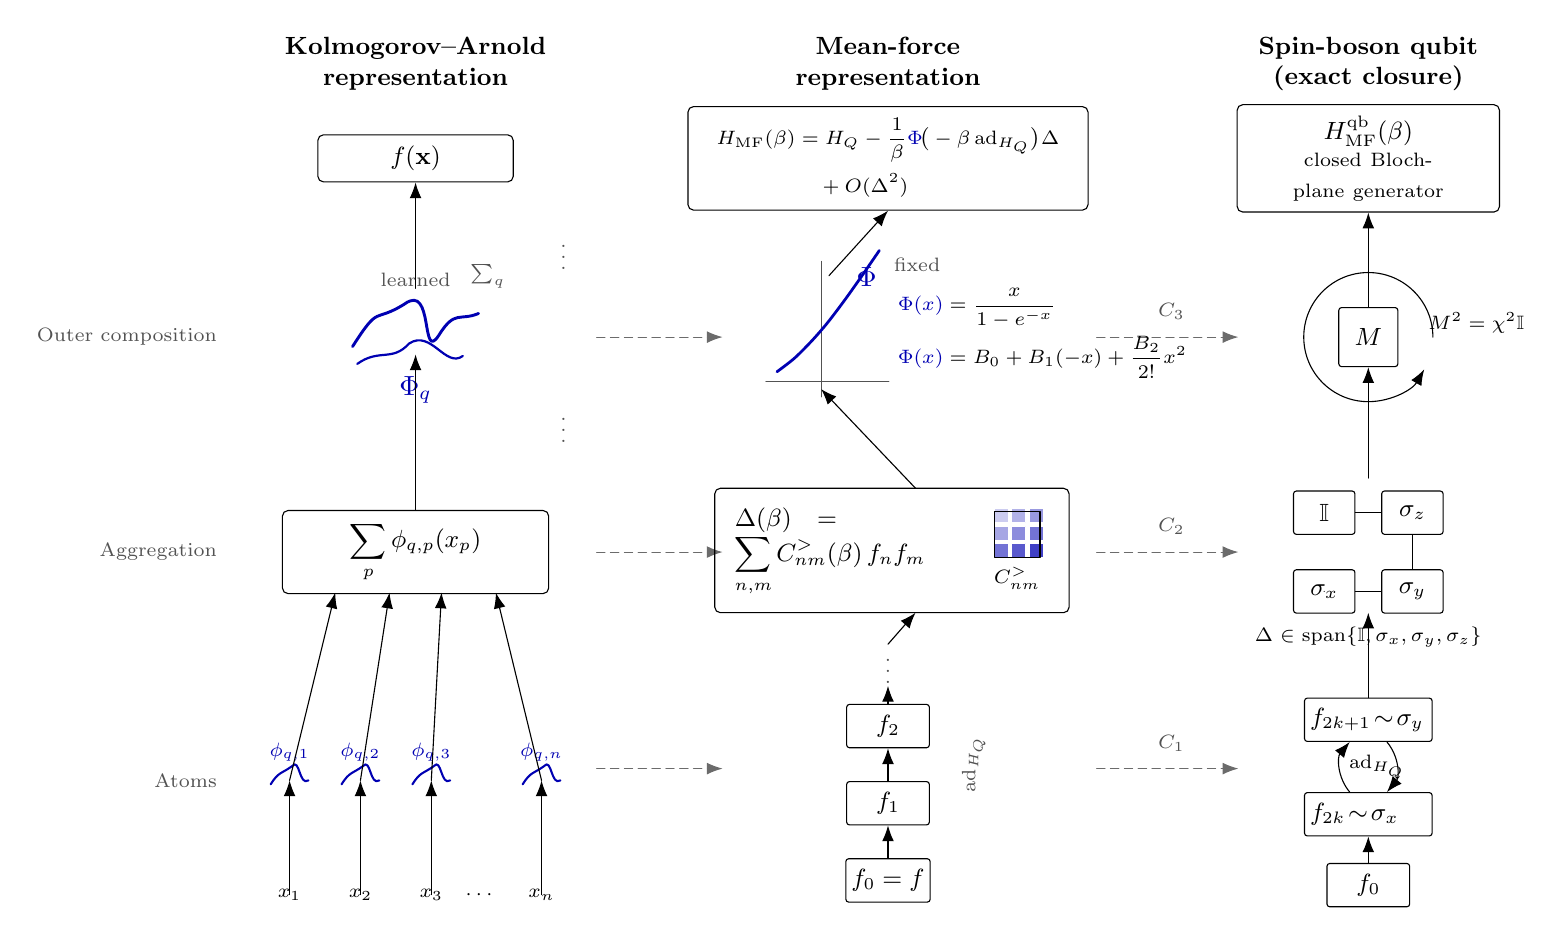
\begin{tikzpicture}[
    x=1cm,
    y=1cm,
    >=Latex,
    font=\small,
    line cap=round,
    line join=round,
    header/.style={font=\bfseries\small, align=center},
    layerlab/.style={font=\scriptsize, text=black!68, anchor=east},
    phimark/.style={font=\normalsize\bfseries, text=accent},
    plainarrow/.style={-{Latex[length=2mm]}, thin},
    corresp/.style={densely dashed, -{Latex[length=2mm]}, thin, draw=black!58},
    orbitnode/.style={
        draw,
        rounded corners=1pt,
        inner sep=2pt,
        minimum width=1.05cm,
        minimum height=0.55cm,
        fill=white
    },
    box/.style={
        draw,
        rounded corners=2pt,
        thin,
        fill=white,
        inner sep=4pt,
        align=center
    },
    smalllab/.style={font=\scriptsize, inner sep=1pt}
]
\colorlet{accent}{blue!70!black}
\colorlet{muted}{black!68}

\def\xL{2.55}
\def\xC{8.55}
\def\xR{14.65}
\def\yIn{0.70}
\def\yAtoms{2.15}
\def\yAgg{5.05}
\def\yOuter{7.78}
\def\yOut{10.05}
\def\yHead{11.25}

% Headers
\node[header] at (\xL,\yHead) {Kolmogorov--Arnold\\representation};
\node[header] at (\xC,\yHead) {Mean-force\\representation};
\node[header] at (\xR,\yHead) {Spin-boson qubit\\(exact closure)};

% Stratum labels
\node[layerlab] at (0.15,\yAtoms) {Atoms};
\node[layerlab] at (0.15,\yAgg) {Aggregation};
\node[layerlab] at (0.15,\yOuter) {Outer composition};

% Horizontal correspondence arrows
\draw[corresp] (4.85,\yAtoms+0.15) -- (6.45,\yAtoms+0.15);
\draw[corresp] (4.85,\yAgg) -- (6.45,\yAgg);
\draw[corresp] (4.85,\yOuter) -- (6.45,\yOuter);
\draw[corresp] (11.20,\yAtoms+0.15) -- (13.00,\yAtoms+0.15);
\draw[corresp] (11.20,\yAgg) -- (13.00,\yAgg);
\draw[corresp] (11.20,\yOuter) -- (13.00,\yOuter);
\node[font=\scriptsize\bfseries, text=muted] at (12.15,\yAtoms+0.47) {$C_1$};
\node[font=\scriptsize\bfseries, text=muted] at (12.15,\yAgg+0.33) {$C_2$};
\node[font=\scriptsize\bfseries, text=muted] at (12.15,\yOuter+0.33) {$C_3$};

% Left column: KAN inputs
\node[box, text width=2.20cm] (outL) at (\xL,\yOut) {$f(\mathbf{x})$};
\node[smalllab, text=muted] at (\xL+1.88,8.90) {$\vdots$};
\node[smalllab, text=muted] at (\xL+1.88,6.70) {$\vdots$};

\coordinate (LPhi) at (\xL,\yOuter);
\draw[accent, line width=1.05pt]
    ($(LPhi)+(-0.80,-0.12)$)
    .. controls +(0.35,0.55) and +(-0.40,-0.25) ..
    ($(LPhi)+(-0.14,0.42)$)
    .. controls +(0.38,0.28) and +(-0.24,-0.38) ..
    ($(LPhi)+(0.30,0.03)$)
    .. controls +(0.20,0.32) and +(-0.24,-0.10) ..
    ($(LPhi)+(0.80,0.30)$);
\draw[accent, line width=0.8pt]
    ($(LPhi)+(-0.74,-0.34)$)
    .. controls +(0.28,0.20) and +(-0.22,-0.24) ..
    ($(LPhi)+(-0.08,-0.08)$)
    .. controls +(0.28,0.18) and +(-0.22,-0.16) ..
    ($(LPhi)+(0.60,-0.24)$);
\node[phimark] at ($(LPhi)+(0,-0.67)$) {$\Phi_q$};
\node[smalllab, text=muted] at ($(LPhi)+(0,0.73)$) {learned};
\draw[plainarrow] ($(LPhi)+(0,0.62)$) -- (outL.south);
\node[smalllab, text=muted] at (\xL+0.92,8.55) {$\sum_q$};

\node[box, text width=3.10cm] (LAgg) at (\xL,\yAgg)
    {$\displaystyle \sum_p \phi_{q,p}(x_p)$};
\draw[plainarrow] (LAgg.north) -- ($(LPhi)+(0,-0.22)$);

\coordinate (x1) at (0.95,\yIn);
\coordinate (x2) at (1.85,\yIn);
\coordinate (x3) at (2.75,\yIn);
\coordinate (xn) at (4.15,\yIn);
\coordinate (p1) at (0.95,\yAtoms);
\coordinate (p2) at (1.85,\yAtoms);
\coordinate (p3) at (2.75,\yAtoms);
\coordinate (pn) at (4.15,\yAtoms);

\node[smalllab] at (x1) {$x_1$};
\node[smalllab] at (x2) {$x_2$};
\node[smalllab] at (x3) {$x_3$};
\node[smalllab] at (3.38,\yIn) {$\cdots$};
\node[smalllab] at (xn) {$x_n$};

\foreach \pt/\lbl in {p1/{\phi_{q,1}},p2/{\phi_{q,2}},p3/{\phi_{q,3}},pn/{\phi_{q,n}}}{
    \draw[accent, line width=0.75pt]
        ($(\pt)+(-0.24,-0.05)$)
        .. controls +(0.10,0.16) and +(-0.14,-0.10) ..
        ($(\pt)+(0.03,0.18)$)
        .. controls +(0.10,0.12) and +(-0.12,-0.08) ..
        ($(\pt)+(0.24,0.00)$);
    \node[smalllab, accent] at ($(\pt)+(0,0.36)$) {$\lbl$};
}

\draw[plainarrow] (x1) -- (p1);
\draw[plainarrow] (x2) -- (p2);
\draw[plainarrow] (x3) -- (p3);
\draw[plainarrow] (xn) -- (pn);
\draw[plainarrow] (p1) -- ($(LAgg.south)+(-1.02,0.02)$);
\draw[plainarrow] (p2) -- ($(LAgg.south)+(-0.33,0.02)$);
\draw[plainarrow] (p3) -- ($(LAgg.south)+(0.33,0.02)$);
\draw[plainarrow] (pn) -- ($(LAgg.south)+(1.02,0.02)$);

% Center column: HMF
\node[box, text width=4.80cm, font=\scriptsize] (outC) at (\xC,\yOut)
    {$\begin{aligned}
        H_{\mathrm{MF}}(\beta) &= H_Q-\frac{1}{\beta}
        {\color{accent}\Phi}\!\big(-\beta\,\mathrm{ad}_{H_Q}\big)\Delta \\
        &\quad + O(\Delta^2)
    \end{aligned}$};

\coordinate (CG) at (7.70,\yOuter);
\draw[muted, thin] ($(CG)+(-0.70,-0.56)$) -- ($(CG)+(0.86,-0.56)$);
\draw[muted, thin] ($(CG)+(0,-0.76)$) -- ($(CG)+(0,0.96)$);
\draw[accent, line width=1.0pt]
    plot[smooth] coordinates {
        ($(CG)+(-0.56,-0.44)$)
        ($(CG)+(-0.34,-0.27)$)
        ($(CG)+(-0.12,-0.05)$)
        ($(CG)+(0.08,0.18)$)
        ($(CG)+(0.30,0.47)$)
        ($(CG)+(0.52,0.78)$)
        ($(CG)+(0.74,1.10)$)
    };
\node[phimark] at (8.28,\yOuter+0.76) {$\Phi$};
\node[smalllab, text=muted] at (8.92,\yOuter+0.92) {fixed};
\node[align=left, anchor=west, font=\scriptsize] (PhiText) at (8.55,\yOuter+0.05)
    {$\textcolor{accent}{\Phi(x)}=\dfrac{x}{1-e^{-x}}$\\[2pt]
     $\textcolor{accent}{\Phi(x)}=B_0 + B_1(-x) + \dfrac{B_2}{2!}x^2$};
\draw[plainarrow] ($(CG)+(0.10,0.78)$) -- (outC.south);

\draw[thin, rounded corners=2pt] (6.35,4.28) rectangle (10.85,5.86);
\node[align=left, text width=2.95cm] at (8.08,\yAgg)
    {$\displaystyle \Delta(\beta)=\sum_{n,m} C^>_{nm}(\beta)\,f_n f_m$};
\foreach \i/\x in {0/9.90,1/10.12,2/10.34}{
    \foreach \j/\y/\shade in {
        0/5.42/20,
        1/5.20/35,
        2/4.98/55
    }{
        \pgfmathtruncatemacro{\mix}{\shade + 10*\i}
    \fill[accent!\mix, draw=white] (\x,\y) rectangle ++(0.18,0.18);
    }
}
\draw[thin] (9.90,4.98) rectangle (10.48,5.56);
\node[smalllab] at (10.19,4.72) {$C^>_{nm}$};
\draw[plainarrow] (8.90,5.86) -- ($(CG)+(0,-0.66)$);

\node[orbitnode] (f0) at (\xC,0.88) {$f_0=f$};
\node[orbitnode] (f1) at (\xC,1.86) {$f_1$};
\node[orbitnode] (f2) at (\xC,2.84) {$f_2$};
\node[smalllab, text=muted] at (\xC,3.64) {$\vdots$};
\draw[plainarrow] (f0) -- (f1);
\draw[plainarrow] (f1) -- (f2);
\draw[plainarrow] (f2) -- (\xC,3.35);
\node[smalllab, rotate=90, text=muted] at (9.64,2.36) {$\mathrm{ad}_{H_Q}$};
\draw[plainarrow] (\xC,3.88) -- (8.90,4.28);

% Right column: exact qubit closure
\node[box, text width=3.05cm] (outR) at (\xR,\yOut)
    {$H_{\mathrm{MF}}^{\mathrm{qb}}(\beta)$\\[-1pt]
    \scriptsize closed Bloch-plane generator};

\node[orbitnode, minimum width=0.75cm, minimum height=0.75cm] (Mnode) at (\xR,\yOuter) {$M$};
\draw[plainarrow] ($(Mnode)+(0.82,0)$) arc[start angle=0,end angle=330,radius=0.82];
\node[smalllab, anchor=west] at (\xR+0.72,\yOuter+0.18) {$M^2=\chi^2\mathbb I$};
\draw[plainarrow] (Mnode.north) -- (outR.south);

\coordinate (qsq) at (\xR,\yAgg);
\node[orbitnode, minimum width=0.78cm] (Id) at (\xR-0.56,\yAgg+0.50) {$\mathbb I$};
\node[orbitnode, minimum width=0.78cm] (Sz) at (\xR+0.56,\yAgg+0.50) {$\sigma_z$};
\node[orbitnode, minimum width=0.78cm] (Sx) at (\xR-0.56,\yAgg-0.50) {$\sigma_x$};
\node[orbitnode, minimum width=0.78cm] (Sy) at (\xR+0.56,\yAgg-0.50) {$\sigma_y$};
\draw[thin] (Id) -- (Sz) -- (Sy) -- (Sx) -- cycle;
\node[smalllab, align=center, text width=3.00cm] at (\xR,\yAgg-1.08)
    {$\Delta \in \mathrm{span}\{\mathbb I,\sigma_x,\sigma_y,\sigma_z\}$};
\draw[plainarrow] (\xR,\yAgg+0.94) -- (Mnode.south);

\node[orbitnode] (q0) at (\xR,0.82) {$f_0$};
\node[orbitnode, text width=1.48cm, minimum width=1.55cm] (qe) at (\xR,1.72)
    {$f_{2k}\!\sim\!\sigma_x$};
\node[orbitnode, text width=1.48cm, minimum width=1.55cm] (qo) at (\xR,2.92)
    {$f_{2k+1}\!\sim\!\sigma_y$};
\draw[plainarrow] (q0) -- (qe);
\draw[plainarrow] (qe) to[bend left=40] node[right=2pt, smalllab] {$\mathrm{ad}_{H_Q}$} (qo);
\draw[plainarrow] (qo) to[bend left=40] (qe);
\draw[plainarrow] (qo.north) -- (\xR,4.28);

\end{tikzpicture}
}
    \caption{Three-layer compositional correspondence between
    Kolmogorov--Arnold representations, the exact Gaussian Hamiltonian of mean
    force, and the spin-boson qubit. Left: a KAN builds a target from
    univariate edge functions $\phi_{q,p}(x_p)$, additive aggregation, and
    outer univariate maps $\Phi_q$. Center: the HMF construction has the same
    layer structure, with adjoint orbit
    $f_n=\mathrm{ad}_{H_Q}^n(f)$, bilinear aggregation
    $\Delta(\beta)=\sum_{n,m} C^>_{nm}(\beta)f_n f_m$, and outer composition by
    the Todd function $\Phi(x)=x/(1-e^{-x})$ fixed analytically by the BCH
    expansion. Right: for the qubit, Conditions (C1)--(C3) close the adjoint
    orbit, bilinear sector, and BCH recombination exactly. The shared
    accent-coloured $\Phi$ highlights the visual rhyme between learned and
    thermodynamically fixed outer composition.}
    \label{fig:kan_hmf_closure}
\end{figure*}

This is more than a family resemblance. The Gaussian HMF construction already
provides the three ingredients usually separated in a compact compositional
model: basis atoms, an aggregation tensor, and a nonlinear composition rule.
The adjoint orbit is a discrete univariate basis in operator space: one
generator, one seed, one orbit index $n$. The matrix $C^>_{nm}(\beta)$ is the
aggregation tensor, but here it is fixed analytically by the bath kernel rather
than learned from data. The Todd/Bernoulli superoperator
\(\Phi(-\beta\,\mathrm{ad}_{H_Q})\), together with the higher BCH nests,
supplies the nonlinear composition rule. Thermodynamics therefore provides both
the architecture and the weights.

Once written in this form, representability failure becomes a precise statement
about model-class insufficiency. If the adjoint orbit or its quadratic and BCH
closures escape $\mathcal A$, the exact reduced generator still exists but no
finite ansatz in that class can carry it without projection. For non-quadratic
continuous-variable potentials the orbit typically expands into the universal
enveloping algebra, so the thermodynamic target outgrows any fixed finite
operator family. That is the same structural obstruction that motivates compact
decompositions in KANs: the universal object exists, but the chosen finite
representation need not be rich enough to realize it.

In that more modest sense the discussion also touches mechanistic
interpretability. Once the layers are explicit, one can inspect which channels
carry the reduced generator and which ones force basis growth. The object being
interpreted here, however, is not a trained network but an exact reduced
equilibrium operator. We now exhibit a case where all three compositional
layers close exactly.

% !TEX root = ../main.tex
\section{Spin-Boson Model as a Closed Reduced Generator}
\label{sec:qubit_closed_generator}\label{subsec:qubit_exact_geometry}

We now exhibit a case where all three compositional layers close exactly in the
spin-boson model~\cite{leggettDynamicsDissipativeTwostate1987,weissQuantumDissipativeSystems2012}.
This is the minimal genuinely noncommuting testbed: the adjoint orbit
terminates into a two-family alternation, the bilinear influence remains in the
Pauli algebra, and the full BCH tower resums to a closed generator. To our
knowledge, this yields the first closed-form Hamiltonian of mean force for a
genuinely noncommuting open quantum system. Earlier exact benchmarks are either
commuting, quadratic/Gaussian, or asymptotic; here the reduced generator stays
inside a finite operator algebra with no approximation at any stage.

Let us first set conventions. During derivation we work in the qubit energy
basis, $\hat{\mathbf n}_s=\hat{\mathbf z}$, and then rewrite the final answer
covariantly in the coupling plane spanned by $\hat{\mathbf n}_s$ and
$\hat{\mathbf f}$. We take
\begin{equation}
    H_Q = \frac{\omega_q}{2}\,\hat{\mathbf n}_s\!\cdot\!\boldsymbol{\sigma},
    \qquad
    f = \hat{\mathbf f}\!\cdot\!\boldsymbol{\sigma},
\end{equation}
with $\hat{\mathbf f}=(s\cos\phi,s\sin\phi,c)$, $c\equiv\cos\theta$,
$s\equiv\sin\theta$. The overall coupling amplitude $g$ is suppressed in
intermediate expressions and reintroduced when discussing scaling.

\subsection{Bath kernels and the symmetrized influence state}
\label{subsec:qubit_influence_state}

The interaction-picture coupling operator is
\begin{equation}
    \tilde f(\tau)=e^{\tau H_Q}fe^{-\tau H_Q}
    = c\sigma_z + f_-e^{\omega_q\tau}\sigma_+ + f_+e^{-\omega_q\tau}\sigma_-,
\end{equation}
with $f_\pm=s e^{\pm i\phi}$. The Pauli algebra then implies that all bath
dependence enters through two real response channels,
\begin{equation}
    \begin{aligned}
    \Sigma_z &\equiv \frac{1}{2}\!\left[R(\omega_q)-R(-\omega_q)\right], \\
    \Sigma_\perp &\equiv \frac{4}{\omega_q}\!\left[
        \cosh\!\left(\frac{\beta\omega_q}{2}\right)\mathcal K(0)
        -e^{-\beta\omega_q/2}\mathcal K(\omega_q)\right].
    \end{aligned}
    \label{eq:bath_kernels_direct}
\end{equation}
The reduced operator can be written in the symmetrized form
$\bar\rho_Q=\Pi^{1/2}e^S\Pi^{1/2}$, with $\Pi=e^{-\beta H_Q}$ and
\begin{equation}
    S=\Delta_0\mathbb I
    +s^2\Sigma_z\,\sigma_z
    -sc\,\Sigma_\perp(\cos\phi\,\sigma_x+\sin\phi\,\sigma_y).
    \label{eq:S_symmetrised_v3}
\end{equation}
Subtracting the scalar piece, $M\equiv S-\Delta_0\mathbb I$, gives an influence
Bloch vector
\begin{equation}
    \mathbf m_S=
    s\Sigma_\perp\hat{\mathbf f}_\perp + s^2(\Sigma_z-\Sigma_\perp)\hat{\mathbf n}_s,
    \label{eq:mS_decomposition}
\end{equation}
where $\hat{\mathbf f}_\perp=(-c\cos\phi,-c\sin\phi,s)$ lies in the coupling
plane and is orthogonal to $\hat{\mathbf f}$.

The corresponding influence magnitude is
\begin{equation}
    \chi=\|\mathbf m_S\|
    = |s|\sqrt{c^2\Sigma_\perp^2+s^2\Sigma_z^2},
    \label{eq:chi_factored}
\end{equation}
and the normalized influence state is
\begin{equation}
    \rho_S=\frac{e^S}{\Tr(e^S)}
    = \frac{1}{2}\!\left[\mathbb I+\tanh\chi\,\hat{\mathbf m}_S\!\cdot\!\boldsymbol{\sigma}\right],
    \qquad
    \hat{\mathbf m}_S=\mathbf m_S/\chi.
    \label{eq:expS_closed}
\end{equation}
Its tilt inside the coupling plane is fixed by the ratio of response channels,
\begin{equation}
    \tan\varphi_S=-\,\frac{c}{s}\,\frac{\Sigma_\perp}{\Sigma_z}.
    \label{eq:phiS_def}
\end{equation}
At this stage the constructive content is already visible: the entire bath has
compressed to two scalar channels and one influence magnitude. The first two
compositional layers have therefore already closed: the adjoint orbit has
collapsed into finitely many Pauli directions, and the bilinear influence has
compressed into a finite set of response coefficients.

\subsection{Closed reduced state and generator}
\label{subsec:qubit_closed_generator}

Recombining the influence state with the bare Gibbs factor yields the reduced
state
\begin{equation}
    \rho_Q = \frac{1}{2}\big[\mathbb I + r_Q \hat{\mathbf m}_Q \cdot \boldsymbol{\sigma}\big],
    \label{eq:rho_matrix_general}
\end{equation}
with Bloch components
\begin{equation}
    m_z = r_Q\cos\varphi_Q,
    \qquad
    m_\perp = r_Q\sin\varphi_Q.
    \label{eq:tilt_angle_def}
\end{equation}
The longitudinal scale is controlled by
\begin{align}
    \Theta &\equiv
    \operatorname{arctanh}\!\big(\gamma(\chi)\,s^2\Sigma_z\big)
    -\frac{\beta\omega_q}{2},
    \label{eq:theta_param} \\
    \gamma(\chi) &\equiv \tanh\chi/\chi,
\end{align}
which gives the exact solution
\begin{align}
    m_z &= \tanh\Theta,
    \label{eq:m_z_solution} \\
    m_\perp &= \tan\varphi_S\!\left(
        m_z\cosh\frac{\beta\omega_q}{2}
        +\sinh\frac{\beta\omega_q}{2}\right).
    \label{eq:bloch_locking_linear}
\end{align}
The final tilt and radius follow as
\begin{equation}
    \tan\varphi_Q = \tan\varphi_S\,
    \frac{m_z + r_0}{\sqrt{1-r_0^2}\;m_z},
    \qquad
    r_0=\tanh\!\left(\frac{\beta\omega_q}{2}\right),
    \label{eq:phiQ_def}
\end{equation}
and
\begin{equation}
    1-r_Q^2
    = \frac{(1-r_0^2)(1-r_S^2)}{(1+r_0 r_S\cos\varphi_S)^2},
    \qquad
    r_S=\tanh\chi.
    \label{eq:rQ_geometric_composition}
\end{equation}
Figure~\ref{fig:bloch_overview} summarizes this Bloch-plane geometry while
Eqs.~\eqref{eq:m_z_solution}--\eqref{eq:rQ_geometric_composition} are being
parsed: the bare Gibbs state, the symmetrized influence state, and the final
reduced state all remain in a single plane fixed by the system and coupling
axes.

\begin{figure}[!t]
    \centering
    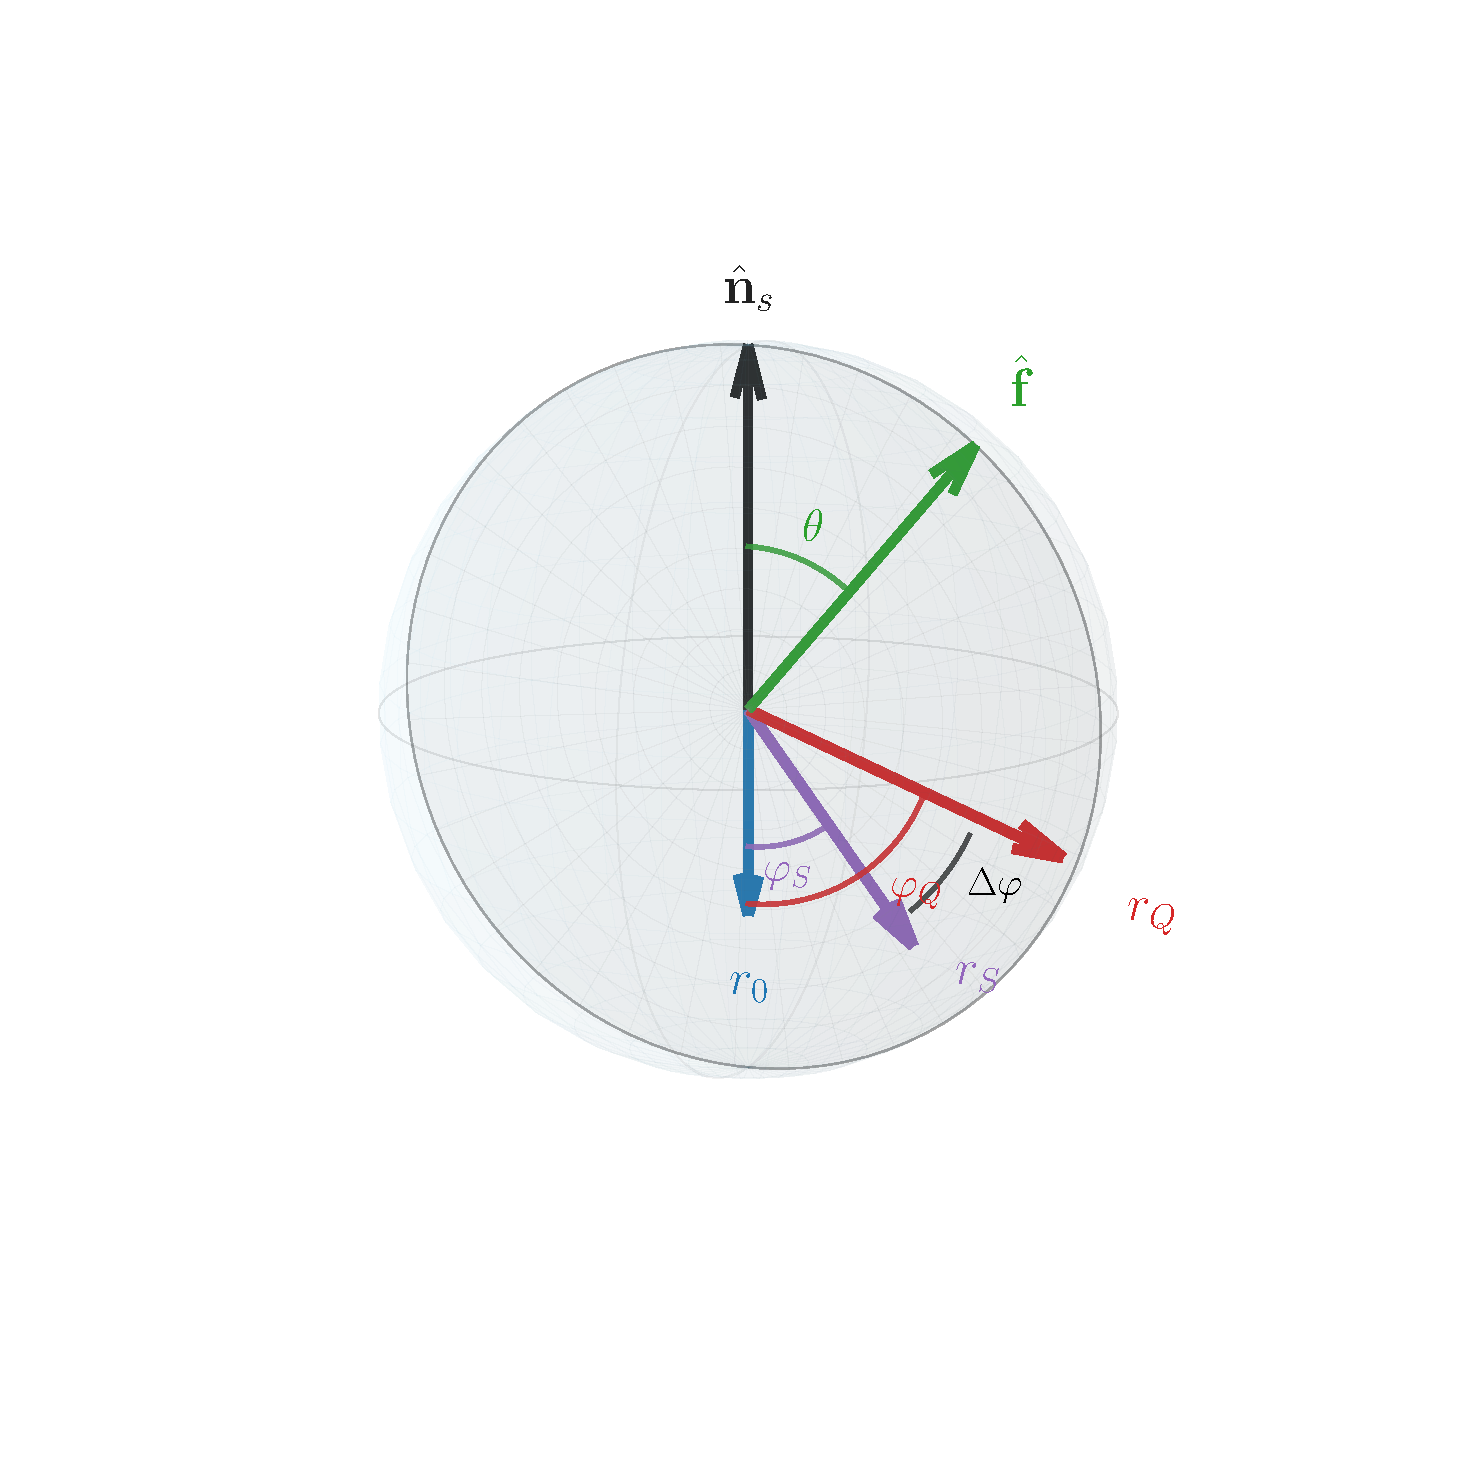
\includegraphics[width=0.84\columnwidth]{../figures/hmf_bloch_3d_overview.pdf}
    \caption{Bloch-plane geometry for the exact qubit construction. The bare
    thermal state has radius $r_0$ (blue), the symmetrized influence state has
    radius $r_S$ and tilt $\varphi_S$ (purple), and the final reduced state has
    radius $r_Q$ and tilt $\varphi_Q$ (red). The exact generator never leaves
    the system--coupling plane.}
    \label{fig:bloch_overview}
\end{figure}

For any full-rank qubit state, the operator logarithm is elementary. Writing
$\hat{\mathbf m}_Q=(m_\perp\cos\phi,m_\perp\sin\phi,m_z)/r_Q$, the exact qubit
Hamiltonian of mean force is therefore
\begin{equation}
    H_{\mathrm{MF}}(\beta)
    = h_0(\beta)\,\mathbb I
    - \frac{1}{\beta}\operatorname{arctanh}(r_Q)\,
      \hat{\mathbf m}_Q\!\cdot\!\boldsymbol{\sigma},
    \label{eq:HMF_qubit_closed_hmf_ai}
\end{equation}
where the scalar $h_0(\beta)$ fixes normalization and carries the additive
identity freedom of the HMF. Equation~\eqref{eq:HMF_qubit_closed_hmf_ai} makes
the closure statement concrete: the exact reduced generator remains inside the
same Bloch-plane operator family throughout, while the bath enters only through
the two response channels $(\Sigma_z,\Sigma_\perp)$ and the influence scale
$\chi$. This is the fully closed instance of the compositional proposition:
the adjoint orbit terminates, the bilinear aggregation closes in the Pauli
algebra, and the nonlinear BCH sector resums because the traceless influence
obeys $M^2=\chi^2\mathbb I$.

% !TEX root = ../main.tex
\section{Physical Regimes of the Mean-Force State}
\label{sec:response_scale}\label{sec:numerical_v6}

The exact qubit solution isolates a single scalar control variable,
\(\chi\), so it is natural to organize the state diagnostics around it.
Reintroducing an explicit dimensionless coupling strength through
\begin{equation}
    K(u)=g^2 K_0(u),
\end{equation}
all response kernels inherit the same quadratic scaling and the influence
magnitude factorizes as
\begin{equation}
    \chi(\beta,g,\theta)=g^2\chi_0(\beta,\theta).
\end{equation}
The entire recombination of bare Gibbs weight and bath influence is therefore
controlled by the universal scalar function
\begin{equation}
    \gamma(\chi)=\frac{\tanh\chi}{\chi}.
    \label{eq:gamma_chi_crossover_v5}
\end{equation}

The exact crossover scale is determined by \(\chi\sim 1\), or equivalently
\begin{equation}
    \chi(\beta,g,\theta)\sim 1
    \qquad \Longleftrightarrow \qquad
    g^2 \sim \chi_0(\beta,\theta)^{-1},
    \label{eq:chi_crossover_condition_v5}
\end{equation}
which defines the coupling scale
\begin{equation}
    g_\star(\beta)=\chi_0(\beta,\theta)^{-1/2}.
    \label{eq:gstar_def_v6}
\end{equation}
No approximation has been made here: \(g_\star(\beta)\) is an exact property of
the reduced generator.

Two benchmark asymptotes remain useful. For \(\chi\ll 1\),
\begin{equation}
    \gamma(\chi)\simeq 1-\frac{\chi^2}{3},
    \label{eq:gamma_weak}
\end{equation}
so the reduced state tracks the bare Gibbs description with perturbative
bath-induced corrections. For \(\chi\gg 1\),
\begin{equation}
    \gamma(\chi)\simeq \chi^{-1},
    \label{eq:gamma_strong}
\end{equation}
so the reduced generator is dominated by the normalized influence direction.
These asymptotes are best read as benchmarks. The main point is that the full
crossover is captured by one response coordinate.

To make these statements concrete we choose the windowed Ohmic spectral density
\begin{equation}
  J(\omega) = g^2\,\omega\,e^{-\omega/\omega_c},
  \qquad \omega\in[0, 2\omega_q],
  \label{eq:J_ohmic_v6}
\end{equation}
with cutoff \(\omega_c=5\omega_q\). The ultraviolet window matches the
finite-mode simulations of the next section, while the exponential cutoff
regularizes the high-frequency tail~\cite{nematiCouplingFunctionBath2022a}.
Having fixed the bath, we set \(\theta=\pi/4\) and \(\omega_q=1\), since the
remaining behavior is already captured by the universal \(\chi\)-scaling.

\begin{figure}[t]
  \centering
  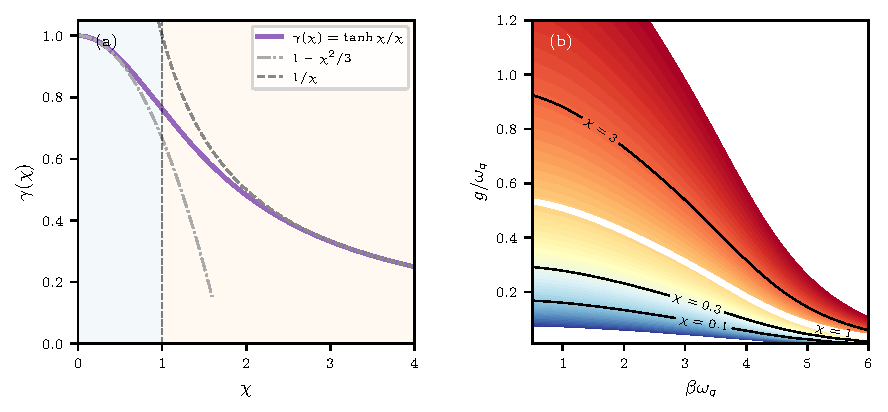
\includegraphics[width=0.48\textwidth]{../figures/hmf_fig1_chi_theory_ab.pdf}
  \caption{Universal crossover structure for the exact qubit mean-force state.
    \textit{Panel~(a)}: Recombination function
    \(\gamma(\chi)=\tanh\chi/\chi\), which interpolates between the small-\(\chi\)
    and large-\(\chi\) benchmarks and makes the \(\chi\sim 1\) crossover
    explicit.
    \textit{Panel~(b)}: Contour map of \(\chi(\beta,g)=g^2\chi_0(\beta)\) for
    the Ohmic bath \eqref{eq:J_ohmic_v6}. The highlighted locus \(\chi=1\)
    defines the exact crossover scale \(g_\star(\beta)=\chi_0(\beta)^{-1/2}\),
    separating weak-response and strongly dressed sectors.}
  \label{fig:chi_theory}
\end{figure}

The same scale organizes the state geometry itself. For a qubit,
\begin{equation}
  \mathcal P_Q = \frac{1}{2}(1+r_Q^2),
\end{equation}
so the Bloch radius \(r_Q\) directly measures the purity of the reduced
equilibrium state. In the exact solution, increasing coupling drives the state
away from the bare thermal radius
\(r_0=\tanh(\beta\omega_q/2)\) and toward a more strongly dressed state. The
effect is most visible at high temperature, where the bare Gibbs state is
nearly mixed and bath-induced structure is easiest to see.

\begin{figure}[t]
  \centering
  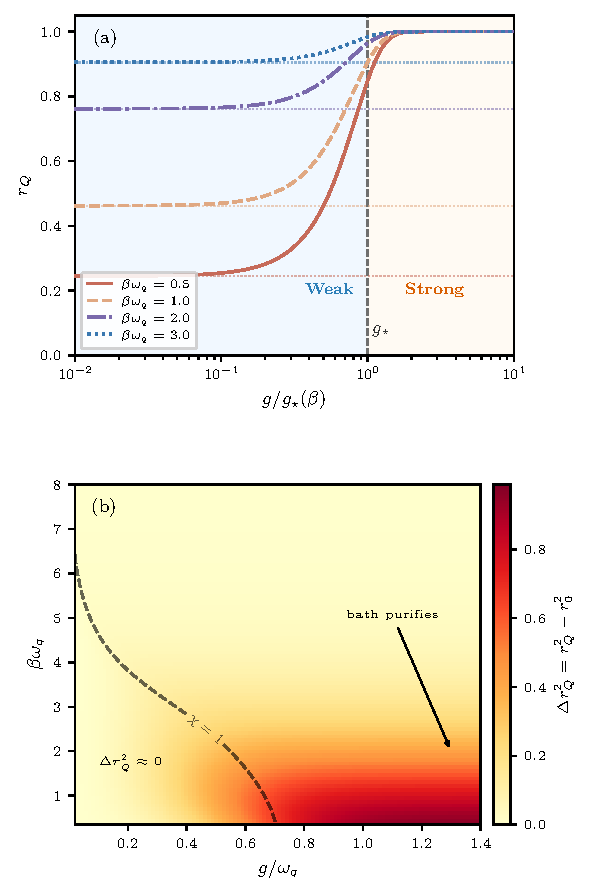
\includegraphics[width=\columnwidth]{../figures/hmf_purity_figure.pdf}
  \caption{Purification diagnostics for the exact qubit mean-force state.
    \textit{Panel~(a)}: Reduced-state Bloch radius \(r_Q\) versus scaled
    coupling \(g/g_\star(\beta)\) for several temperatures. Dotted horizontal
    lines mark the corresponding bare thermal radii \(r_0\); the dressed state
    moves away from the bare Gibbs value most sharply near the crossover.
    \textit{Panel~(b)}: Purity excess
    \(\Delta r_Q^2 \equiv r_Q^2-r_0^2\) over the \((g,\beta)\) plane. The
    dashed contour \(\chi=1\) tracks the same crossover scale seen in
    Fig.~\ref{fig:chi_theory}.}
  \label{fig:purity_figure}
\end{figure}

The same coordinate also controls how rapidly the reduced state changes.
Differentiating the exact Bloch components shows that the angle susceptibility
and radius gradient peak at fixed values of \(\chi\), namely
\(\chi_{\mathrm{peak},\varphi}\approx 0.42\) and
\(\chi_{\mathrm{peak},r}\approx 0.85\) for the Ohmic example used below. After
rescaling the coupling as \(g/g_\star(\beta)\), these peaks align across
temperatures. The alignment is not a numerical accident; it is the statement
that the response scale is intrinsic to the exact reduced generator.

\begin{figure}[t]
  \centering
  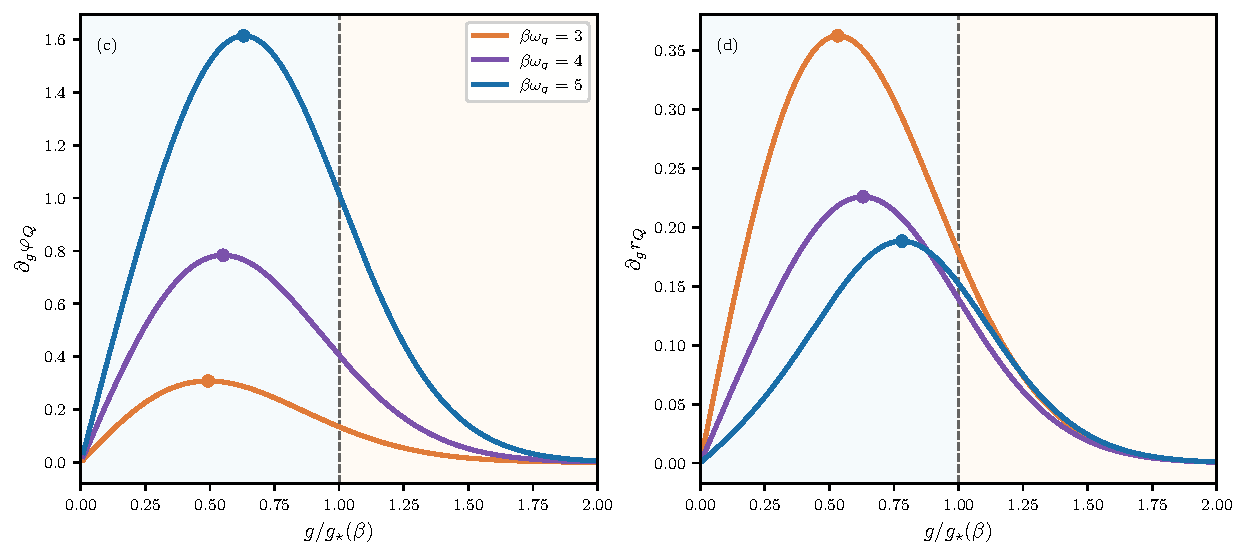
\includegraphics[width=\columnwidth]{../figures/hmf_fig1_chi_theory_cd_v3.pdf}
  \caption{Response susceptibilities of the exact reduced state.
    \textit{Panel~(c)}: Tilt susceptibility \(\partial_g\varphi_Q\) versus the
    scaled coupling \(g/g_\star(\beta)\).
    \textit{Panel~(d)}: Radius gradient \(\partial_g r_Q\) on the same scale.
    In both cases the peak positions collapse across temperatures and sit near,
    but not exactly on, the crossover line. The exact reduced state is therefore
    most sensitive to bath dressing in a narrow band around \(\chi\sim 1\).}
  \label{fig:chi_susceptibility}
\end{figure}

These figures do two jobs for the remainder of the paper. First, they make the
exact-state geometry visible: crossover, purification, and susceptibility are
all controlled by the same scalar response coordinate. Second, they identify
the narrow region where a compact reduced generator changes most rapidly. That
is precisely the region where finite-basis numerics become the hardest to keep
inside a restricted representational class.

% !TEX root = ../main.tex
\section{Representability Diagnostics in Truncated Baths}
\label{sec:numerical_results}

The physical-regime diagnostics above identify where the exact reduced state
changes most rapidly. We now ask how finite-basis numerics behave across that
same region. The exact qubit solution developed in the previous section depends
on the bath only through response data at three frequencies,
\(\omega\in\{0,\pm\omega_q\}\). To test it we
compare against exact diagonalization (ED) of a truncated spin-boson model,
where the qubit is coupled to \(N_\omega\) harmonic oscillators and each mode
is represented with a finite Fock cutoff \(n_{\max}\). A useful feature of this
comparison is that the analytic kernel integrals can be evaluated in two ways:
using the full continuum spectral density (the \emph{continuous analytic}
branch) or using the same discrete mode set seen by ED (the \emph{discrete
analytic} branch). The comparison therefore tests not only the exact reduced
generator but also whether a chosen finite numerical representation can realize
the same compact reduced description.

Figure~\ref{fig:ed_vs_analytic} compares the excited-state population
\(p_{11}\) across coupling strengths and inverse temperatures for
\(N_\omega=40\) modes. At small \(\chi\), all three curves coincide. As the
system crosses the exact response scale \(\chi\sim 1\), the analytic
predictions separate from ED. The key point is that the discrete analytic
branch does \emph{not} follow the numerical deviation: it bends back toward the
continuum benchmark. This shows that the exact HMF theory is already correct
for the discrete mode set itself. The discrepancy is therefore not a failure of
the theory, nor a finite-mode artifact.

The remaining gap is a representability bottleneck in the truncated Hilbert
space. In the large-response regime the coupled system approaches a displaced,
polaron-like ground state, and faithfully representing that state requires
\(n_{\max}\gtrsim |\alpha_k|^2\) for each displaced mode
\(\alpha_k\sim g_k/\omega_k\). Once \(\chi\gtrsim 1\), the chosen Fock cutoff
can no longer support the required occupations. ED is then trapped in a model
class that is too small to contain the exact dressed equilibrium state. In the
language of the compositional discussion above, the target reduced generator is
known exactly but the chosen finite representation lacks the capacity to
realize it.

\begin{figure}[t]
  \centering
  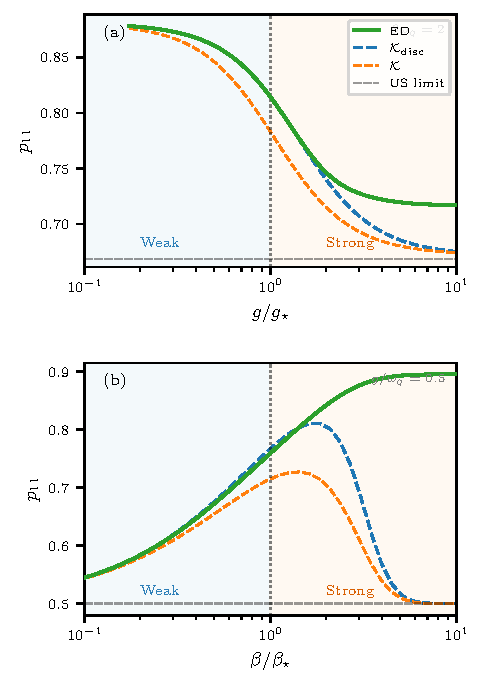
\includegraphics[width=0.48\textwidth]{../figures/hmf_fig2_ed_vs_analytic.pdf}
  \caption{Excited-state population \(p_{11}\) across the exact response scale
    for \(N_\omega=40\) modes. Green solid: ED. Blue dashed: discrete analytic
    theory using the same mode set. Orange dotted: continuum analytic theory.
    Dashed horizontal lines mark the large-response benchmark \(p_\infty\). The
    gap between ED and the analytic branches is a representability failure of
    the truncated basis, not a breakdown of the exact reduced generator.}
  \label{fig:ed_vs_analytic}
\end{figure}

The same interpretation explains the bandwidth sensitivity in
Fig.~\ref{fig:bandwidth_convergence}. Varying the spectral window changes how
the displacement load is distributed over the available modes. As the system is
pushed across the response scale, the required occupations grow and the
available Fock space is exhausted. The sharp peak in cutoff sensitivity is
therefore a direct signature of the finite basis hitting its representational
boundary.

\begin{figure}[t]
  \centering
  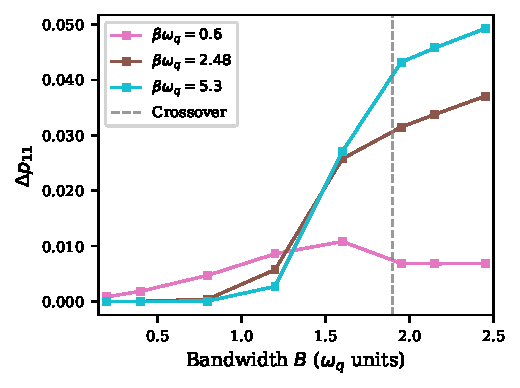
\includegraphics[width=0.48\textwidth]{../figures/hmf_fig3_bandwidth_convergence.pdf}
  \caption{Cutoff sensitivity
    \(\Delta p_{11}\equiv |p_{11}(n_{\max}=4)-p_{11}(n_{\max}=6)|\) as a
    function of spectral bandwidth \(B\) in units of \(\omega_q\). The
    sensitivity peak marks the onset of the representability bottleneck: beyond
    this point the truncated basis can no longer accommodate the mode
    occupations required by the exact dressed state.}
  \label{fig:bandwidth_convergence}
\end{figure}

The numerical message is therefore narrower, and stronger, than a generic
``agreement with simulation'' claim. The analytic HMF provides the correct
reduced target for both discrete and continuous baths. The observed numerical
deviations diagnose when a chosen finite model class is no longer expressive
enough to realize that target.

% !TEX root = ../main.tex
\section{Discussion}
\label{sec:discussion}

This paper makes four connected points. First, the Hamiltonian of mean force is
best viewed as a constructive reduced generator, not merely as a formal
logarithm. Second, in the Gaussian sector this constructive question reduces to
a closure problem for the adjoint chain generated by \(H_Q\) and the coupling
operator. Third, the same structure can be written as an explicit
compositional architecture, which is why the KAN comparison can be made
formally rather than rhetorically. Fourth, the same closure logic explains both
exact solvability and the failure modes of finite-basis numerics.

\subsection*{Closure and constructive reduced generators}

The central algebraic result is that representability of the HMF inside a
restricted operator family has an exact answer. Conditions (C1)--(C3) separate
the problem into three layers: whether repeated adjoint action grows the
operator basis, whether the Gaussian influence remains inside that basis, and
whether the BCH recombination generates further operators. When all three hold,
the reduced equilibrium admits an exact finite generator. When they fail, the
failure is structural rather than computational: the reduced state can still be
computed, but not compressed losslessly into the proposed ansatz.

This makes the closure theorem useful beyond the present example. It turns the
usual question ``can we evaluate the reduced state?'' into the sharper question
``which operator family is large enough to contain the exact reduced
generator?'' In that form, the theorem is already a guide to controlled
approximation. One may truncate the operator side without approximating the bath
side, and the resulting error has a clear interpretation as model-class error.

\subsection*{The qubit as an exact noncommuting benchmark}

For the spin-boson qubit, closure is exact. The reduced generator remains in
the Bloch plane determined by the system axis and the coupling axis, and the
entire bath compresses to two scalar response channels together with the
influence magnitude \(\chi\). To our knowledge, this makes
Eq.~\eqref{eq:HMF_qubit_closed_hmf_ai} the first closed-form Hamiltonian of
mean force for a genuinely noncommuting open quantum system. Earlier exact
benchmarks are either commuting, quadratic/Gaussian, or asymptotic. Here none
of those simplifications is doing the work. The work is done by complete
closure of the compositional architecture itself.

That mechanism is worth isolating. The adjoint orbit terminates into a
two-family alternation, the bilinear influence remains in the Pauli algebra,
and the nonlinear BCH tower resums because the traceless influence obeys
$M^2=\chi^2\mathbb I$. Figure~\ref{fig:bloch_overview} is the geometric
signature of that fact: bare state, influence state, and final reduced state
all remain inside one Bloch plane. What should generalize to larger systems is
not the specific Pauli formulas but the separation between bath data and
operator growth, together with the question of whether every layer of that
structure still closes.

\subsection*{Representability bottlenecks and finite-resource inference}

The numerical diagnostics sharpen the interpretation. ED disagrees with the
analytic prediction not when the theory becomes inaccurate, but when the chosen
finite basis is no longer expressive enough to realize the exact dressed state.
The response scale \(\chi\sim 1\) marks the onset of this bottleneck in the
examples studied here. In other words, the crossover is simultaneously physical
and representational: it tracks both the reorganization of the reduced state
and the point at which a restricted model class begins to fail.

This is why the distinction between discrete analytic and numerical ED matters.
Once the discrete analytic branch peels away from ED and returns toward the
continuum benchmark, the problem is no longer one of physics missed by the
generator. It is one of structure missed by the basis. That diagnosis is useful
well beyond this example, because many approximate methods in open-system
physics are precisely choices of tractable operator or Hilbert-space classes.

\subsection*{Compositional architectures, representation cost, and KANs}

Recent work on representation cost emphasizes that exact state descriptions are
less useful than explicit generators that expose what must be retained under
coarse-graining~\cite{mccaulCostComplexity2026}. The HMF offers a concrete
equilibrium realization of that principle. The partial trace hides a large
environment inside a reduced state; closure determines whether that hidden
structure can still be recast as a compact generator.

The strengthened KAN correspondence is not decorative. Kolmogorov--Arnold
networks ask when multivariate dependence can be realized by a compact
composition of univariate edge functions and additive aggregation
~\cite{liuKANKolmogorovArnoldNetworks2024}. The Gaussian HMF problem already
has that architecture built in. The adjoint orbit is the univariate basis in
operator space, the ordered-kernel matrix $C^>_{nm}(\beta)$ is the aggregation
tensor, and the Todd/Bernoulli BCH resummation is the nonlinear composition
rule. Here those objects are not learned by optimization; they are supplied in
closed form by equilibrium thermodynamics.

In that dictionary, the operator ansatz $\mathcal A$ is the model class and
closure failure is model-class insufficiency. The exact reduced generator still
exists, but a fixed finite representation cannot realize it without projection.
That is why the non-quadratic continuous-variable obstruction and the
finite-basis numerical bottleneck belong in the same discussion: both are
instances of a universal target outgrowing the chosen compact representation.
Mechanistic interpretability enters only after that point. Once the layers are
explicit, one can inspect which channels carry the reduced generator and which
ones force basis growth.

\subsection*{Limitations and outlook}

The main analytic restriction is Gaussianity. The quenched representation itself
is more general, but the exact collapse of the influence to a bilinear operator
depends on the bath cumulant hierarchy truncating at second order. Beyond that
sector, higher cumulants generate higher operator monomials and the closure
problem becomes correspondingly richer.

Within the Gaussian sector, the next natural targets are multi-qubit systems and
other finite-dimensional models where the adjoint chain generates nontrivial
many-body operator content. There the central question is no longer whether an
HMF exists, but how rapidly operator growth escapes a chosen locality class. In
that sense the present qubit solution is a starting point for a broader study
of constructive reduced generators in interacting systems. A second direction
is methodological: once the reduced generator is written as an explicit
compositional object, one can ask which approximate schemes preserve that
architecture and which ones merely fit the reduced state after the fact.

% !TEX root = ../Hamiltonian_of_mean_force.tex
\section{Acknowledgments}
Several thanks are in order. First to William J. Handley, for demonstrating by example the power of the new science. Never again shall I mistake mental athleticism for real scientific vision. Naturally, the engines of this new methodology deserve credit. Thanks to Claude, Gemini, and Barry for extensive discussions and assistance. The present work would have been impossible without their input, despite the fact they are shiftless layabouts who will happily tell you the sky is green. Speaking of limited but developing intelligences, the author's unborn son has his eternal gratitude for electing to delay their drop until this manuscript was completed. 


\appendix
\setcounter{secnumdepth}{2}
\input{sections/10_appendix}
\input{sections/11_appendix_algebraic}
% !TEX root = ../Hamiltonian_of_mean_force.tex
\section{Exact Qubit Solution in the Ladder Basis}
\label{app:qubit_ladder_derivation}

We provide the manual derivation of the exact qubit mean-force state using the ladder basis $\sigma_\pm$. Starting from the interaction-picture operator product
\begin{equation}
\begin{aligned}
    \tilde{f}(\tau)\tilde{f}(\tau')
    &= \Big[c^2 + s^2\cosh\big(\omega_q(\tau-\tau')\big)\Big]\mathbb{I} \\
    &\quad + s^2\sinh\big(\omega_q(\tau-\tau')\big)\sigma_z \\
    &\quad + c f_- \left(e^{\omega_q\tau'} - e^{\omega_q\tau}\right)\sigma_+ \\
    &\quad + c f_+ \left(e^{-\omega_q\tau} - e^{-\omega_q\tau'}\right)\sigma_-,
\end{aligned}
\end{equation}
the influence exponent $\Delta = \int_0^\beta d\tau \int_0^\tau d\tau' K(\tau-\tau') \tilde{f}(\tau)\tilde{f}(\tau')$ evaluates to
\begin{equation}
    \Delta = \Delta_0 \mathbb{I} + \Delta_z \sigma_z + \Delta_+ \sigma_+ + \Delta_- \sigma_-,
\end{equation}
with coefficients
\begin{align}
    \Delta_z &= s^2 \Sigma_z, \\
    \Delta_\pm &= -2 c f_\mp \Sigma_\pm,
\end{align}
where $f_\pm = s e^{\pm i \phi_f}$ and the primitive integrals are
\begin{align}
    \Sigma_z &= \frac{1}{2}\left[R(\omega_q) - R(-\omega_q)\right], \\
    \Sigma_\pm &= \frac{1}{\omega_q} \left[\big(1 + e^{\pm\beta\omega_q}\big)\mathcal{K}(0) - 2\mathcal{K}(\pm\omega_q)\right].
\end{align}
The unnormalised state is $\bar\rho_Q = e^{-(\beta\omega_q/2) \sigma_z} e^\Delta$. To find the normalized state and its Bloch vector, we perform a symmetric decomposition
\begin{equation}
    \bar\rho_Q = \Pi^{1/2} e^S \Pi^{1/2}, \qquad S = \Pi^{1/2} \Delta \Pi^{-1/2}
\end{equation}
where $\Pi = e^{-\beta \omega_q \sigma_z / 2}$. Using $\Pi^{1/2} \sigma_\pm \Pi^{-1/2} = e^{\mp \beta\omega_q/2} \sigma_\pm$, the symmetric influence operator $S$ becomes
\begin{equation}
    S = \Delta_0 \mathbb{I} + \Delta_z \sigma_z + (\Delta_+ e^{-\beta\omega_q/2} \sigma_+ + \Delta_- e^{\beta\omega_q/2} \sigma_-).
\end{equation}
Substituting the expressions for $\Delta_\pm$ and using the KMS relation
\begin{equation}
    \Sigma_- = e^{-\beta\omega_q} \Sigma_+,
    \label{eq:kms_sigma_relation}
\end{equation}
we define the real symmetrised transverse response
\begin{equation}
    \Sigma_\perp \equiv 2 e^{-\beta\omega_q/2} \Sigma_+ = 2 e^{\beta\omega_q/2} \Sigma_-.
\end{equation}
The transverse coefficients then simplify to
\begin{equation}
    \Delta_+ e^{-\beta\omega_q/2} = -c s e^{-i \phi_f} (2 e^{-\beta\omega_q/2} \Sigma_+) = -c s e^{-i\phi_f} \Sigma_\perp,
\end{equation}
with $\Delta_\perp \equiv -c s \Sigma_\perp$. 
Recombining the ladder operators into Cartesian form, we obtain
\begin{equation}
    S = \Delta_0 \mathbb{I} + \Delta_z \sigma_z + \Delta_\perp (\sigma_x \cos\phi_f + \sigma_y \sin\phi_f),
\end{equation}
which is the generator of a rotation around an axis in the coupling plane. The influence magnitude $\chi = \sqrt{\Delta_z^2 + \Delta_\perp^2}$ determines the exponential $e^S = \cosh\chi (\mathbb{I} + \gamma M)$ with $\gamma = \tanh\chi/\chi$ and $M = S - \Delta_0 \mathbb{I}$. The final state $\rho_Q = Z_Q^{-1} \Pi^{1/2} e^S \Pi^{1/2}$ follows by direct matrix multiplication, yielding Eq.~\eqref{eq:rho_matrix_general} in the main text.


\bibliography{../../literature/references_new,../tex/hmf_ai_refs}

\end{document}
